\section{Implémentation}

\begin{figure}[ht]
  \centering
  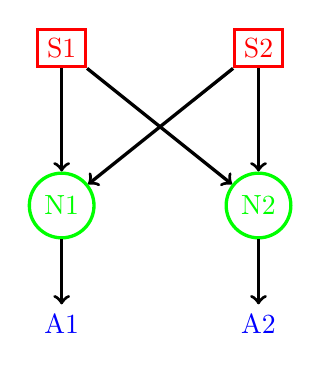
\begin{tikzpicture}[scale=0.5]
 \tikzset{directed/.style={->}} 
  \node[color=blue] (A1) at (0,0) {A1};
  \node[color=blue] (A2) at (5,0) {A2};
  \node[draw, circle, very thick, color=green] (N1) at (0,3) {N1};
  \node[draw, circle, very thick, color=green] (N2) at (5,3) {N2};
  \node[draw, very thick, color=red] (S1) at (0,7) {S1};
  \node[draw, very thick, color=red] (S2) at (5,7) {S2};
  \draw[very thick, directed] (S1) -- (N1);
  \draw[very thick, directed] (S2) -- (N1);
  \draw[very thick, directed] (S1) -- (N2);
  \draw[very thick, directed] (S2) -- (N2);
  \draw[very thick, directed] (N1) -- (A1);
  \draw[very thick, directed] (N2) -- (A2);
\end{tikzpicture}

  \caption{Réseau de neurone à deux neurones}
  \label{graphInit}
\end{figure}

\paragraph{}
Nous pouvons voir sur le schéma \ref{graphInit} que trois types d'objets sont
présents dans notre conception d'un réseau de neurones:\\
\begin{description}
  \item[Les stimuli] Réalisés en rouge sur le schéma, ils génèrent les signaux
    qui activent les premiers neurones et ainsi active le réseau.
  \item[Les actions] Affichés en bleu sur le schéma, elles sont les sorties de
    notre système, elles correspondent à la décision effectué par notre réseau.
  \item[Les neurones] Cœur même du réseau, ils sont là pour effectuer la prise
    de décision en fonction des entrées qu'ils possèdent.
\end{description}

\paragraph{}
Ces trois éléments sont donc la base de notre réseau. Ainsi notre classe correspondant
à un réseau de neurones stockera une liste de stimuli, une liste de réactions et une
liste des neurones constituant le réseau.

\paragraph{}
Il a ensuite fallu déterminer la façon de parcourir tous les neurones pour les
mettre à jour. Cette réflexion a fait émerger deux méthodes. Ces methodes
avaient un impacte sur l'implementation de la classe neurone. \\

\begin{enumerate}
  \item La première consistait en partant des réactions à remonter de façon
    récursive le réseau de neurones afin de récupérer les informations pour
    calculer si oui ou non les réactions ont été activitées. Ces méthodes impliquées
    que chaque neurone est accés à l'ensemble de ces entrées afin de les
    interroger pour savoir si ils ont été activés.
  \item La seconde consistait en partant des stimuli à propager les informations
    d'activation jusqu'aux réactions. Dans cette méthode quand un neurone a calculé
    si oui ou non il a été activé, il prévient alors l'ensemble de ces sorties de
    son status. Un neurone recevant une information d'une de ces entrées la
    sauvegarde et si il a reçu l'ensemble des états de ces entrées alors il calcul
    son propre état et le progage de la même maniére.
\end{enumerate}

La seconde solution a été choisi car elle semblait plus intuitif sur le
façon dont le réseau est parcouru (des stimuli vers les réactions). Avec
l'implémentation choisi, on remarque pour que le réseau soit bien valide,
il ne doit pas avoir des cycles dans le réseau. En effet, si il existe un
cycle il devient alors impossible de calculer les états des neurones
appartenant au cycle car chaque neurone a besoin des états des autres neurones du
cycle.

\paragraph{}
Ne souhaitant pas attribuer aux neurones des caractéristiques qui ne leur étaient
pas nécessaires, nous nous sommes demandé ce qui était intrinsèque au
fonctionnement de l'entité et ce qui relevait de la particularité de notre
réseau. Après réflexion nous sommes arrivé à déterminer comme cœur du neurone, les
parties suivantes:\\

\begin{description}
<<<<<<< HEAD
  \item[Nom] Chaque neurone est doté d'un nom qui permettra de le distinguer
    lors de l'envoi de chaque valeur vers les neurones concernés
  \item[Poids] Chaque neurone va pondérer chacune de ses entrées. Ces poids
    sont stockés dans un dictionnaire avec comme clé le nom du neurone et
    comme valeur le poids qui lui est associé.
  \item[Sorties] La liste des neurones et des reactions connecté à la sortie
    du neurone.
  \item[Inhibiteur] Permet de savoir si le neurone est un inhibiteur où non.
  \item[Taux d'apprentissage] Le taux de variation des poids du neurone.
\end{description}

\paragraph{}
%TODO Apprentissage


